\documentclass[12pt, a4paper]{article}

% --- Pakiety ---
\usepackage[utf8]{inputenc}
\usepackage[T1]{fontenc}
\usepackage[polish]{babel}
\usepackage{geometry}
\usepackage{amsmath}
\usepackage{amssymb}
\usepackage{graphicx}
\usepackage{booktabs}
\usepackage{siunitx}
\usepackage{caption}
\usepackage{subcaption}
\usepackage{float}
\usepackage{hyperref}
\usepackage{xcolor}
\usepackage{array}
\usepackage{multirow}
\usepackage{fancyhdr}

% --- Marginesy ---
\geometry{
    top=2.5cm,
    bottom=2.5cm,
    left=2.5cm,
    right=2.5cm,
    footskip=2cm
}

% --- Stopka ---
\pagestyle{fancy}
\fancyhf{}
\renewcommand{\headrulewidth}{0pt}
\renewcommand{\footrulewidth}{0.4pt}
\fancyfoot[R]{
\includegraphics[height=0.8cm]{lumon.pdf}}

% --- Konfiguracja siunitx ---
\sisetup{
    output-decimal-marker = {,},
    separate-uncertainty = true
}

% --- Dane raportu ---
\newcommand{\tytul}{Pomiar prędkości dźwięku w metalach metodą echa ultradźwiękowego}
\newcommand{\codeword}{Zurich}
\newcommand{\nrCwiczenia}{F9}
\newcommand{\autor}{Karol Peszek}
\newcommand{\nrGrupy}{A}
\newcommand{\dataWykonania}{10 listopada 2026} % TODO: sprawdzić datę pomiarów

% --- Tytuł dokumentu ---
\title{
    \large I Pracownia Fizyczna \\[0.5em]
    \textbf{Ćwiczenie \nrCwiczenia} \\[0.3em]
    \LARGE \tytul\space''\codeword''
}
\author{
    \autor\\
     Grupa \nrGrupy}
\date{
    Data wykonania pomiarów: \dataWykonania\\
}

% =============================================
\begin{document}
% =============================================

\maketitle
\thispagestyle{empty}
\newpage

% -------------------------------------------
\section{Cel ćwiczenia}
% -------------------------------------------

W niniejszej pracy wyznaczono prędkość podłużnej fali ultradźwiękowej w mosiądzu, stali
i~aluminium metodą echa ultradźwiękowego. Dla czterech próbek każdego materiału o grubościach
ok.\ 10--30~mm zmierzono na oscyloskopie czasy dotarcia do głowicy odbiorczej impulsu
bezpośredniego i~kolejnych ech, a prędkość wyznaczono z~nachylenia prostej $s(t)$ dopasowanej
do drogi impulsu w~funkcji czasu. Z~mas i~wymiarów próbek wyznaczono gęstości materiałów,
a z~gęstości i~prędkości --- moduły Younga. Wyniki porównano z~wartościami tablicowymi.

% -------------------------------------------
\section{Wstęp teoretyczny}
% -------------------------------------------

\subsection{Fale sprężyste w ciele stałym}

Ciało stałe przeciwstawia się zarówno zmianie objętości (ściśliwość), jak i~zmianie
kształtu (sztywność), dlatego mogą się w~nim rozchodzić fale podłużne, w~których cząstki
drgają wzdłuż kierunku rozchodzenia się fali, i~poprzeczne, w~których drgają prostopadle
do niego~\cite{skrypt}. Falę harmoniczną biegnącą wzdłuż osi $x$ opisuje równanie
\begin{equation}
    y = A\cos\left[\omega\left(t - \frac{x}{v}\right)\right],
    \label{eq:fala}
\end{equation}
gdzie $A$ --- amplituda, $\omega$ --- częstość kołowa, $v = \lambda f$ --- prędkość
rozchodzenia się fali, $\lambda$ --- długość fali, $f$ --- częstotliwość. Fale o~częstotliwości
powyżej ok.\ 20~kHz, niesłyszalne dla człowieka, nazywa się ultradźwiękami.

\subsection{Prędkość fali podłużnej w pręcie}

Rozważa się pręt o~gęstości $\rho$ i~polu przekroju $S$, ułożony wzdłuż osi $x$. Odkształcenie
pręta przenoszą naprężenia $\sigma$, a element pręta między przekrojami $x$ i~$x + \Delta x$
(Rysunek~\ref{fig:element}) przemieszcza się o~$\xi(x, t)$.

\begin{figure}[H]
    \centering
    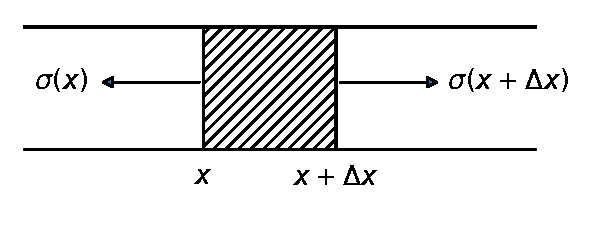
\includegraphics[width=0.55\textwidth]{rod_element.pdf}
    \caption{Naprężenia działające na element odkształconego pręta. Na podstawie~\cite{skrypt}.}
    \label{fig:element}
\end{figure}

Równanie ruchu tego elementu ma postać
\begin{equation}
    \rho S \Delta x \frac{\partial^2 \xi}{\partial t^2} = S\sigma(x + \Delta x) - S\sigma(x),
    \label{eq:ruch}
\end{equation}
skąd w~granicy $\Delta x \to 0$
\begin{equation}
    \rho \frac{\partial^2 \xi}{\partial t^2} = \frac{\partial \sigma}{\partial x}.
    \label{eq:ruch_gr}
\end{equation}
Zgodnie z~prawem Hooke'a naprężenie jest proporcjonalne do odkształcenia względnego:
\begin{equation}
    \sigma = E\varepsilon, \qquad \varepsilon = \frac{\partial \xi}{\partial x},
    \label{eq:hooke}
\end{equation}
gdzie $E$ --- moduł Younga. Podstawienie~\eqref{eq:hooke} do~\eqref{eq:ruch_gr} daje
równanie falowe
\begin{equation}
    \frac{\partial^2 \xi}{\partial t^2} = \frac{E}{\rho}\frac{\partial^2 \xi}{\partial x^2},
    \label{eq:falowe}
\end{equation}
z~którego, przez porównanie z~ogólnym równaniem falowym, prędkość fali podłużnej
w~cienkim pręcie wynosi~\cite{skrypt}
\begin{equation}
    v_\parallel^\text{pręt} = \sqrt{\frac{E}{\rho}}.
    \label{eq:u_pret}
\end{equation}

\subsection{Fale poprzeczne i współczynnik Poissona}

W~podobny sposób wyprowadza się prędkość fali poprzecznej,
\begin{equation}
    v_\perp = \sqrt{\frac{G}{\rho}},
    \label{eq:u_poprz}
\end{equation}
gdzie $G$ --- moduł sztywności, wiążący naprężenie ścinające $\tau$ z~kątem ścinania
$\theta$: $\tau = G\theta$. Wydłużeniu ciała towarzyszy zmniejszenie jego wymiarów
poprzecznych; stosunek względnego skrócenia poprzecznego do względnego wydłużenia to
współczynnik Poissona $\nu$. Dla ciał izotropowych~\cite{skrypt}
\begin{equation}
    G = \frac{E}{2(1 + \nu)}, \qquad
    v_\perp = \sqrt{\frac{E}{2\rho(1 + \nu)}}.
    \label{eq:G}
\end{equation}

\subsection{Fala podłużna w ośrodku o dużych rozmiarach poprzecznych}

Wzór~\eqref{eq:u_pret} zakłada, że pręt może swobodnie zmieniać swoje wymiary poprzeczne.
Gdy rozmiary poprzeczne ośrodka są znacznie większe od długości fali, każdy element objętości
odkształca się tylko w~kierunku podłużnym: skróceniu poprzecznemu przeciwdziała otaczający
materiał, ośrodek jest efektywnie sztywniejszy, a prędkość fali podłużnej wynosi~\cite{skrypt}
\begin{equation}
    v_\parallel = \sqrt{\frac{E(1 - \nu)}{\rho(1 + \nu)(1 - 2\nu)}}
    = v_\parallel^\text{pręt}\sqrt{f(\nu)}, \qquad
    f(\nu) = \frac{1 - \nu}{(1 + \nu)(1 - 2\nu)}.
    \label{eq:u_osr}
\end{equation}
Dla badanych metali $\nu = 0{,}29$--$0{,}34$, więc $f(\nu) = 1{,}31$--$1{,}54$, a prędkość
$v_\parallel$ jest o~14--24\,\% większa od $v_\parallel^\text{pręt}$.

Z~prędkości i~gęstości bezpośrednio wynika moduł podłużny (moduł fali w~ośrodku nieograniczonym)
\begin{equation}
    M = \rho v_\parallel^2 = E f(\nu),
    \label{eq:M}
\end{equation}
a moduł Younga dopiero po przyjęciu współczynnika Poissona:
\begin{equation}
    E = \frac{M}{f(\nu)} = \rho v_\parallel^2\,\frac{(1 + \nu)(1 - 2\nu)}{1 - \nu}.
    \label{eq:E}
\end{equation}
Współczynnik $\nu$ można wyznaczyć bez tablic ze stosunku prędkości fal poprzecznej
i~podłużnej w~ośrodku, który z~wzorów~\eqref{eq:G} i~\eqref{eq:u_osr} wynosi
\begin{equation}
    \left(\frac{v_\perp}{v_\parallel}\right)^2 = \frac{1 - 2\nu}{2(1 - \nu)}.
    \label{eq:nu}
\end{equation}

Dla ultradźwięków o~częstotliwościach rzędu megaherców długość fali w~metalach wynosi kilka
milimetrów, mniej niż średnica badanych próbek (19--25~mm). Częstotliwości głowic nie mierzono,
dlatego to, który z~wzorów~\eqref{eq:u_pret} i~\eqref{eq:u_osr} opisuje próbki, rozstrzyga się
na podstawie wyników (podsekcja~\ref{sec:predkosc}).

\subsection{Metoda echa ultradźwiękowego}

Próbkę o~grubości $l$ umieszcza się między dwiema głowicami ultradźwiękowymi. Głowica
nadawcza zamienia krótki impuls elektryczny z~generatora na impuls ultradźwiękowy, który
przechodzi przez próbkę i~jest rejestrowany przez głowicę odbiorczą. Część energii impulsu
odbija się od powierzchni próbki stykającej się z~głowicą odbiorczą, wraca do głowicy
nadawczej, odbija się ponownie i~po raz drugi dociera do głowicy odbiorczej. Na ekranie
oscyloskopu powstaje ciąg równoodległych impulsów o~wykładniczo malejących amplitudach
(Rysunek~\ref{fig:echo}): pierwszy odpowiada przejściu bezpośredniemu, kolejne --- echom~\cite{skrypt}.

\begin{figure}[H]
    \centering
    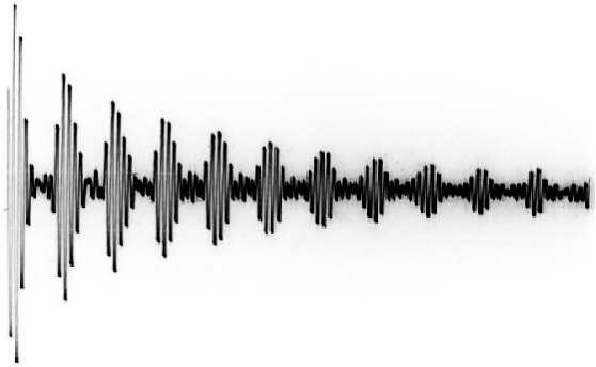
\includegraphics[width=0.6\textwidth]{echo.pdf}
    \caption{Prawidłowy obraz ciągu sygnałów echa ultradźwiękowego na ekranie oscyloskopu
             dla próbki stalowej. Źródło:~\cite{skrypt}.}
    \label{fig:echo}
\end{figure}

Każde kolejne echo przebywa w~próbce dodatkową drogę $2l$. Jeśli $n = 1$ oznacza impuls
bezpośredni, a $n = 2, 3, \dots$ kolejne echa, droga $n$-tego impulsu w~próbce wynosi
\begin{equation}
    s_n = (2n - 1)\,l.
    \label{eq:droga}
\end{equation}
Czas $t_n$ odczytany na oscyloskopie liczy się od chwili wyzwolenia generatora, więc oprócz
czasu przelotu przez próbkę zawiera opóźnienie $\delta$ (czas przejścia impulsu przez głowice,
warstwę oleju i~przewody). Grubość warstwy oleju i~siła docisku mogą się zmieniać między
próbkami, więc opóźnienie $\delta_i$ przypisuje się każdej próbce osobno:
\begin{equation}
    t_n = \frac{s_n}{v_\parallel} + \delta_i = \tau_i\,(2n - 1) + \delta_i,
    \qquad \tau_i = \frac{l_i}{v_\parallel},
    \label{eq:prosta}
\end{equation}
gdzie $\tau_i$ --- czas przejścia impulsu przez grubość próbki $i$. Zależność $t_n$ od $(2n-1)$
jest liniowa; z~jej nachylenia wynika prędkość $v_\parallel = l_i/\tau_i$, a opóźnienie trafia
do wyrazu wolnego i~nie wpływa na wynik.

Gęstość walcowej próbki o~masie $m$, średnicy $d$ i~grubości $l$ wynosi
\begin{equation}
    \rho = \frac{4m}{\pi d^2 l}.
    \label{eq:rho}
\end{equation}

\subsection{Przyjęte wartości}

Wartości tablicowe gęstości, modułu Younga i~prędkości fali podłużnej zestawiono
w~Tabeli~\ref{tab:tablica}. Skrypt nie podaje współczynników Poissona, potrzebnych we
wzorach~\eqref{eq:u_osr} i~\eqref{eq:E}. Według~\cite{poisson} wynoszą one dla aluminium
$0{,}32$--$0{,}35$ (czyste aluminium $0{,}334$), dla mosiądzu $0{,}331$ (mosiądz 70-30) --
$0{,}357$ (mosiądz lany) i~dla stali $0{,}265$ (staliwo) -- $0{,}305$ (stal nierdzewna 18-8).
Skład próbek nie jest znany, dlatego przyjęto $\nu = 0{,}33$ dla aluminium, $0{,}34$ dla
mosiądzu i~$0{,}29$ dla stali, z~niepewnością $u_\nu = 0{,}02$ równą połowie rozrzutu między
gatunkami.

Wartościom tablicowym podanym jako pojedyncza liczba przypisano niepewność równą połowie
ostatniej podanej cyfry ($u_\rho = 50$~kg/m$^3$, $u_v = 5$~m/s, $u_E = 0{,}05 \cdot 10^{10}$~Pa),
a podanym jako przedział --- połowę jego szerokości. W~całym sprawozdaniu rozdzielczości
przyrządów, połowy przedziałów i~$u_\nu$ traktuje się jednakowo, jako niepewności standardowe
bez dzielenia przez $\sqrt{3}$; jest to wariant zachowawczy.

\begin{table}[H]
    \centering
    \caption{Dane akustyczne metali w~temperaturze $20^{\circ}$C~\cite{skrypt} i~przyjęte
             współczynniki Poissona~\cite{poisson}.}
    \label{tab:tablica}
    \begin{tabular}{lcccc}
        \toprule
        Materiał & {$\rho$ [$10^3$ kg/m$^3$]} & {$E$ [$10^{10}$ Pa]} & {$v_\parallel$ [m/s]} & {$\nu$} \\
        \midrule
        mosiądz   & 8,1 & 10,3      & 3830        & $0{,}34 \pm 0{,}02$ \\
        stal      & 7,8 & 21,5      & 5900--6000  & $0{,}29 \pm 0{,}02$ \\
        aluminium & 2,7 & 6,2--7,3  & 6320        & $0{,}33 \pm 0{,}02$ \\
        \bottomrule
    \end{tabular}
\end{table}

% -------------------------------------------
\section{Opis układu pomiarowego}
% -------------------------------------------

Schemat blokowy układu przedstawiono na Rysunku~\ref{fig:schemat}, a jego zdjęcie na
Rysunku~\ref{fig:uklad}. Dwie głowice ultradźwiękowe $G1$ i~$G2$ są zamocowane w~statywie
jedna nad drugą. Badaną próbkę $M$ kładzie się na dolnej głowicy, która może się lekko
przechylać i~dopasowuje się do ewentualnej nierównoległości podstaw próbki, a od góry dociska
się ją górną głowicą. Impuls prostokątny z~generatora $IG$ trafia do głowicy nadawczej
i~równocześnie na wejście oscyloskopu $O$, gdzie wyzwala podstawę czasu; sygnał głowicy
odbiorczej trafia na drugie wejście oscyloskopu~\cite{skrypt}.

\begin{figure}[H]
    \centering
    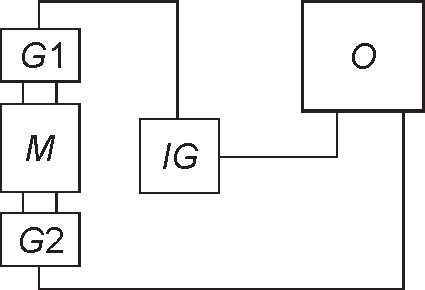
\includegraphics[width=0.4\textwidth]{schema.pdf}
    \caption{Schemat blokowy układu: $G1$, $G2$ --- głowice ultradźwiękowe, $M$ --- próbka,
             $IG$ --- impulsowy generator wysokiej częstotliwości, $O$ --- oscyloskop.
             Źródło:~\cite{skrypt}.}
    \label{fig:schemat}
\end{figure}

\begin{figure}[H]
    \centering
    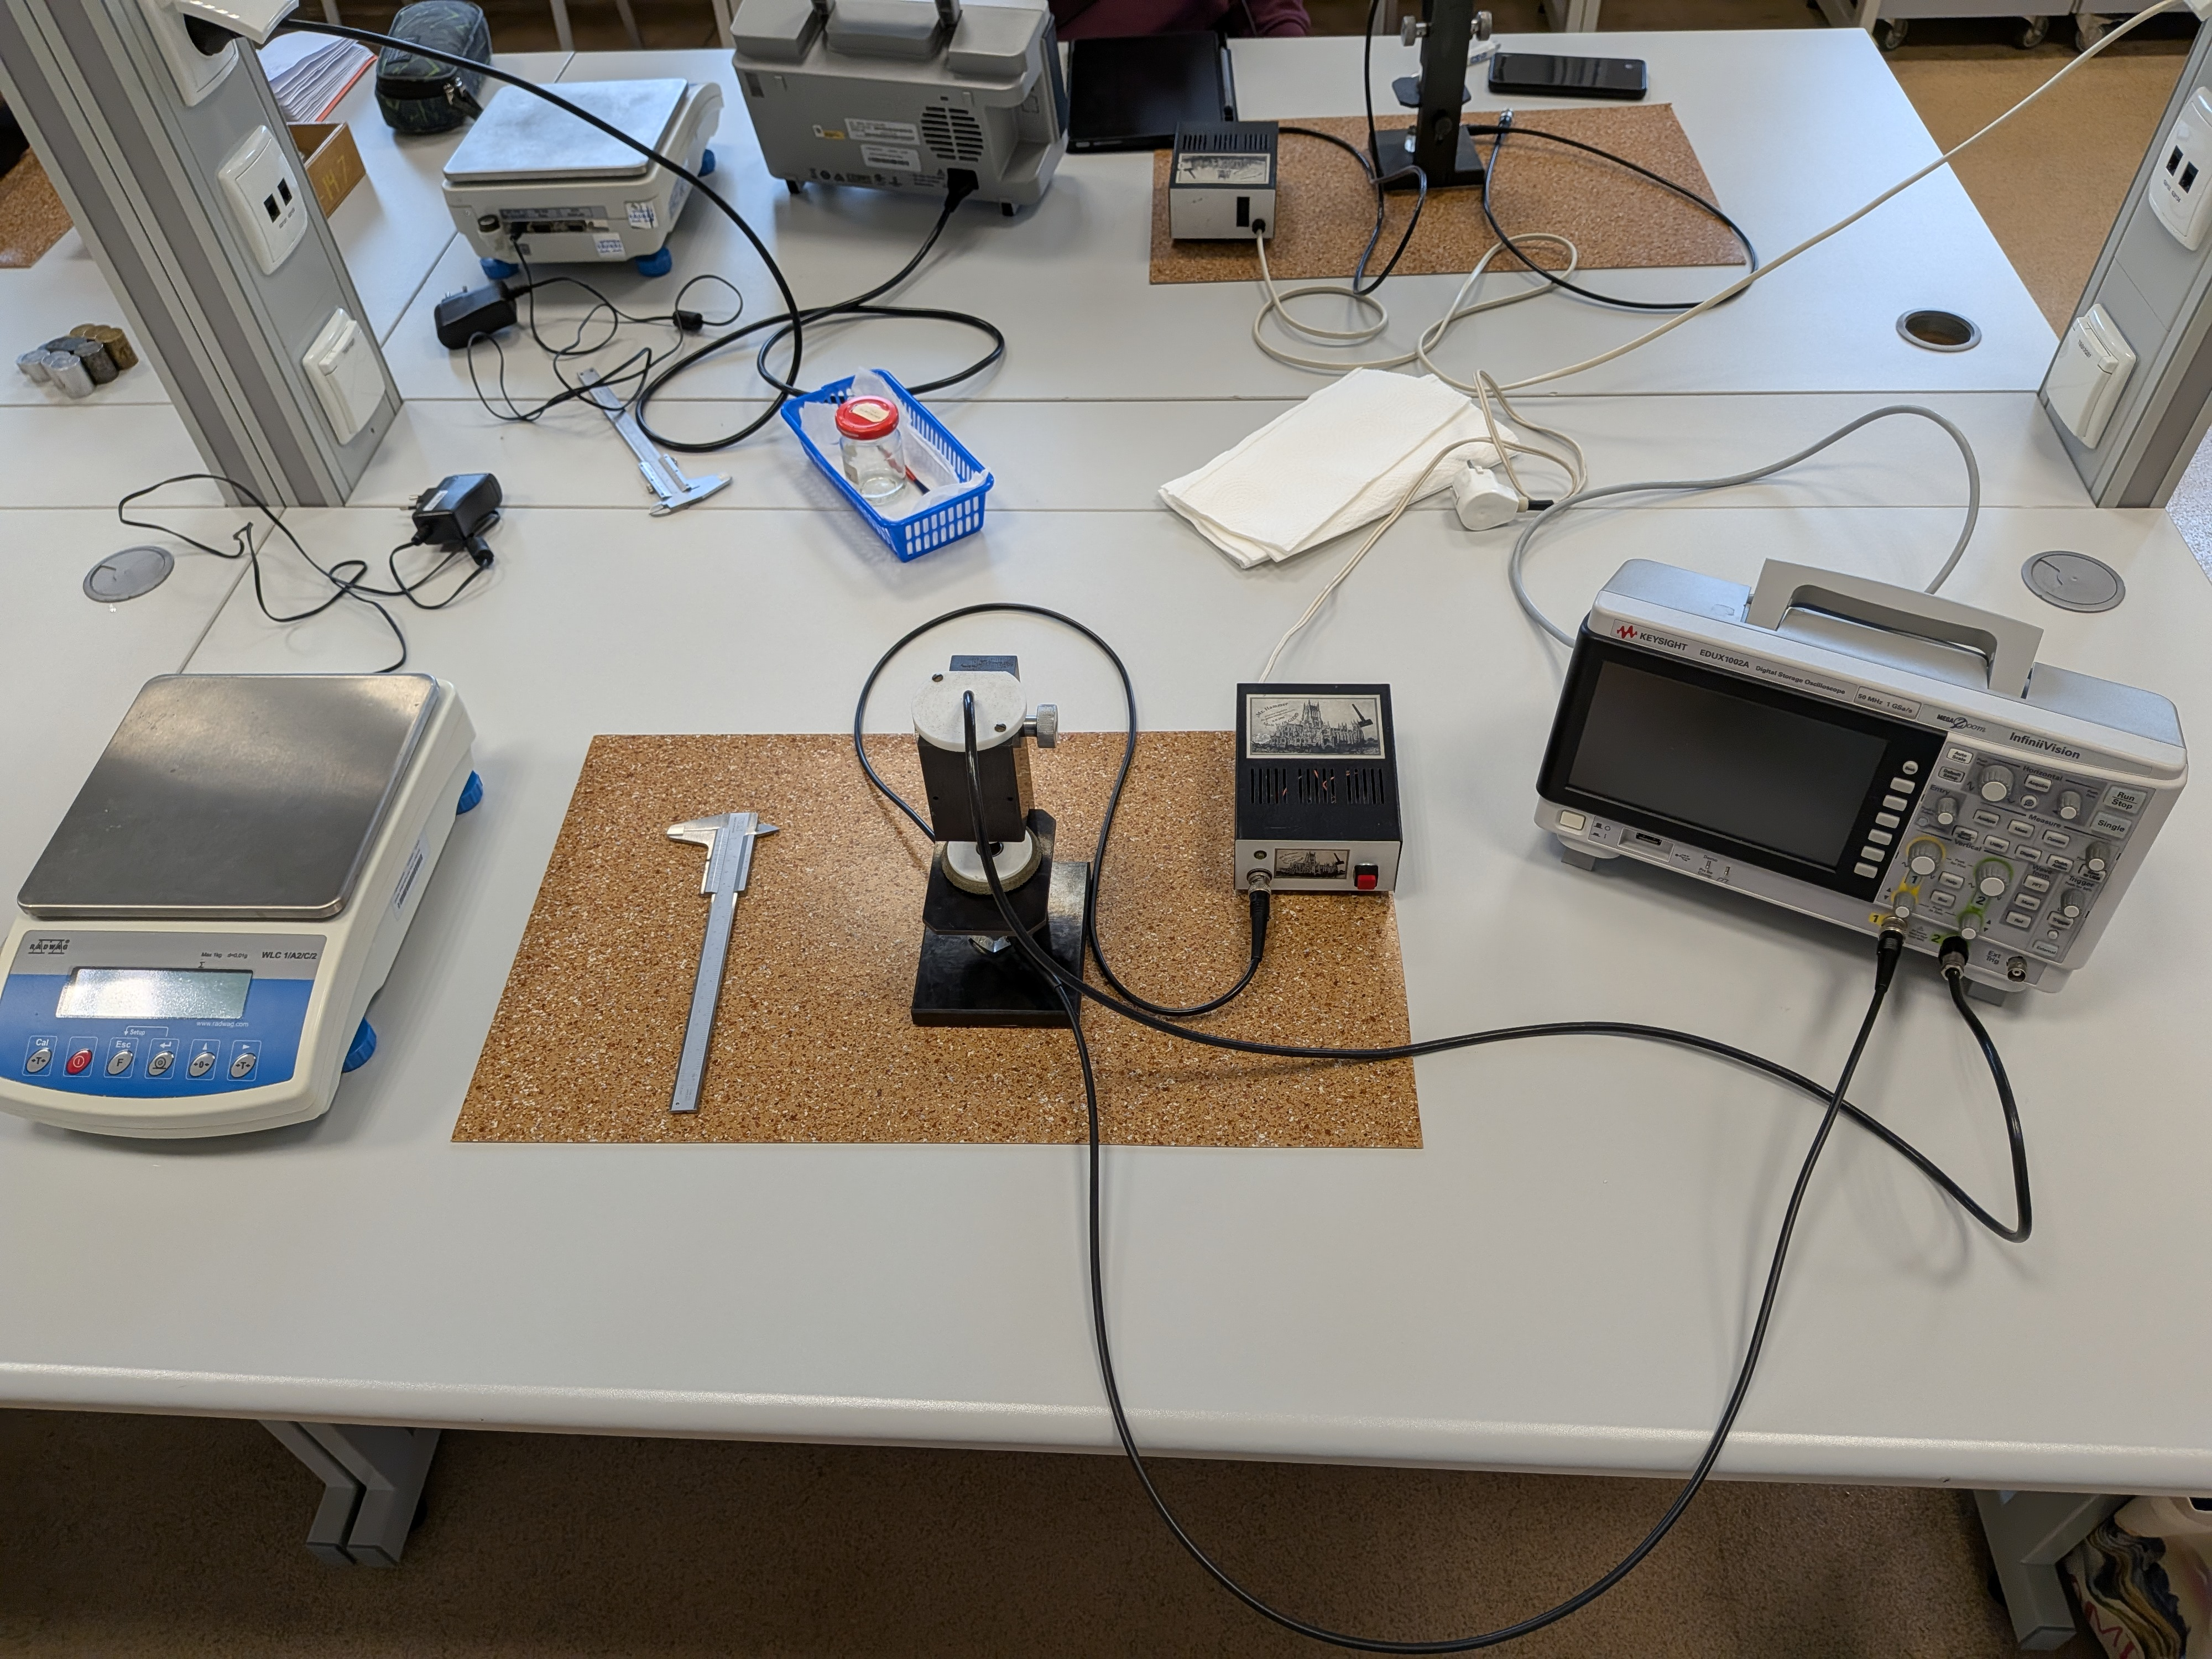
\includegraphics[width=0.85\textwidth]{schema.jpg}
    \caption{Układ pomiarowy: statyw z~głowicami ultradźwiękowymi (w~środku), generator
             impulsów (obok statywu), oscyloskop Keysight EDUX1002A (z~prawej), waga
             laboratoryjna Radwag (z~lewej) i~suwmiarka.}
    \label{fig:uklad}
\end{figure}

Wykorzystano:
\begin{itemize}
    \item dwie głowice ultradźwiękowe zamocowane w~statywie;
    \item impulsowy generator wysokiej częstotliwości;
    \item oscyloskop cyfrowy Keysight EDUX1002A (pasmo 50~MHz, próbkowanie 1~GSa/s); czasy
          impulsów odczytywano z~niepewnością $u_t = 0{,}1$~µs;
    \item 12 walcowych próbek: po cztery z~mosiądzu, stali i~aluminium (skrypt wymaga trzech),
          o~grubościach ok.\ 10, 19--20, 25 i~30~mm;
    \item suwmiarkę o~rozdzielczości $0{,}05$~mm do pomiaru grubości próbek, $u_l = 0{,}05$~mm;
    \item wagę laboratoryjną Radwag WLC~1/A2/C/2 (obciążenie maksymalne 1~kg, działka
          $d = 0{,}01$~g), $u_m = 0{,}01$~g;
    \item olej do smarowania podstaw próbek, poprawiający przyleganie głowic.
\end{itemize}

% -------------------------------------------
\section{Procedura pomiarowa}
% -------------------------------------------

\subsection{Wymiary i masy próbek}

Próbki ponumerowano od 1 do 12 (1--4 --- mosiądz, 5--8 --- stal, 9--12 --- aluminium,
w~każdym materiale od najcieńszej). Grubość i~średnicę każdej próbki zmierzono suwmiarką,
a masę zważono na wadze laboratoryjnej.

\subsection{Czasy przelotu impulsów}

Podstawy próbki posmarowano lekko olejem, próbkę umieszczono na dolnej głowicy i~dociśnięto
górną. Podstawę czasu i~wzmocnienie oscyloskopu ustawiono tak, aby na ekranie był widoczny
ciąg równoodległych impulsów o~wykładniczo malejących amplitudach (Rysunek~\ref{fig:echo}).
Następnie odczytano czasy $t_1, \dots, t_5$ impulsu bezpośredniego i~kolejnych czterech ech,
liczone od chwili wyzwolenia generatora. Za chwilę dotarcia impulsu przyjęto położenie jego
najwyższego maksimum. Przesuwano podstawę czasu tak, aby to maksimum znalazło się na
pionowej osi środkowej ekranu, po powiększeniu skali czasu dla dokładniejszego ustawienia,
i~odczytywano przesunięcie (offset) podstawy czasu.
Dla próbek 7, 8 i~12 piąty impuls, a dla próbki 10 czwarty i~piąty, miały amplitudę zbyt
małą do odczytu, więc zmierzono tylko trzy lub cztery czasy. Pomiar powtórzono dla
wszystkich 12 próbek.

% -------------------------------------------
\section{Wyniki pomiarów}
% -------------------------------------------

Niepewność pomiaru grubości i~średnicy próbek wynosi $u_l = u_d = 0{,}05$~mm (rozdzielczość suwmiarki),
masy $u_m = 0{,}01$~g (działka wagi), a odczytu czasu na oscyloskopie $u_t = 0{,}1$~µs.

\subsection{Wymiary i masy próbek}

Grubości, średnice i~masy wszystkich próbek zestawiono w~Tabeli~\ref{tab:probki}.

\begin{table}[H]
    \centering
    \caption{Grubości $l$, średnice $d$ i~masy $m$ próbek. Niepewności: $u_l = u_d = 0{,}05$~mm,
             $u_m = 0{,}01$~g.}
    \label{tab:probki}
    \begin{tabular}{clS[table-format=2.2]S[table-format=2.2]S[table-format=3.2]}
        \toprule
        Nr & Materiał & {$l$ [mm]} & {$d$ [mm]} & {$m$ [g]} \\
        \midrule
        1  & mosiądz   & 9.55  & 18.90 & 22.86  \\
        2  & mosiądz   & 19.85 & 24.90 & 80.55  \\
        3  & mosiądz   & 24.70 & 24.90 & 101.16 \\
        4  & mosiądz   & 30.00 & 24.90 & 122.35 \\
        \midrule
        5  & stal      & 10.00 & 19.75 & 24.37  \\
        6  & stal      & 19.00 & 24.95 & 72.35  \\
        7  & stal      & 25.20 & 24.15 & 90.04  \\
        8  & stal      & 30.20 & 24.90 & 114.95 \\
        \midrule
        9  & aluminium & 9.20  & 20.00 & 8.17   \\
        10 & aluminium & 19.00 & 25.15 & 26.41  \\
        11 & aluminium & 24.80 & 24.85 & 33.65  \\
        12 & aluminium & 29.90 & 24.90 & 40.58  \\
        \bottomrule
    \end{tabular}
\end{table}

\subsection{Czasy przelotu impulsów}

Czasy $t_n$ impulsu bezpośredniego ($n = 1$) i~kolejnych ech ($n = 2, \dots, 5$), liczone od
wyzwolenia generatora, zestawiono w~Tabeli~\ref{tab:czasy}. Kreska oznacza impuls o~amplitudzie
zbyt małej do odczytu.

\begin{table}[H]
    \centering
    \caption{Czasy $t_n$ dotarcia $n$-tego impulsu do głowicy odbiorczej. Niepewność
             $u_t = 0{,}1$~µs.}
    \label{tab:czasy}
    \begin{tabular}{clS[table-format=1.2]S[table-format=2.2]S[table-format=2.2]S[table-format=2.2]S[table-format=2.2]}
        \toprule
        Nr & Materiał & {$t_1$ [µs]} & {$t_2$ [µs]} & {$t_3$ [µs]} & {$t_4$ [µs]} & {$t_5$ [µs]} \\
        \midrule
        1  & mosiądz   & 3.44 & 7.76  & 12.07 & 16.39 & 20.93 \\
        2  & mosiądz   & 5.68 & 14.53 & 23.70 & 32.55 & 41.45 \\
        3  & mosiądz   & 6.78 & 17.80 & 29.11 & 40.12 & 51.18 \\
        4  & mosiądz   & 7.94 & 21.76 & 35.38 & 48.76 & 61.93 \\
        \midrule
        5  & stal      & 2.90 & 6.30  & 9.70  & 13.10 & 16.48 \\
        6  & stal      & 4.20 & 10.68 & 17.05 & 23.42 & 29.69 \\
        7  & stal      & 5.50 & 13.97 & 22.36 & 31.02 & {--}  \\
        8  & stal      & 6.20 & 16.48 & 26.54 & 36.86 & {--}  \\
        \midrule
        9  & aluminium & 2.65 & 5.52  & 8.36  & 11.21 & 14.06 \\
        10 & aluminium & 4.20 & 10.09 & 16.00 & {--}  & {--}  \\
        11 & aluminium & 5.10 & 12.79 & 20.71 & 28.33 & 36.32 \\
        12 & aluminium & 5.90 & 15.20 & 24.27 & 33.86 & {--}  \\
        \bottomrule
    \end{tabular}
\end{table}

Na podstawie wzoru~\eqref{eq:droga} każdemu czasowi $t_n$ przypisano drogę impulsu w~próbce
$s_n = (2n-1)\,l$, z~niepewnością $u(s_n) = (2n-1)\,u_l$. Zależności $s(t)$ dla mosiądzu, stali
i~aluminium przedstawiono na Rysunkach~\ref{fig:brass_raw}--\ref{fig:aluminium_raw}.

\begin{figure}[H]
    \centering
    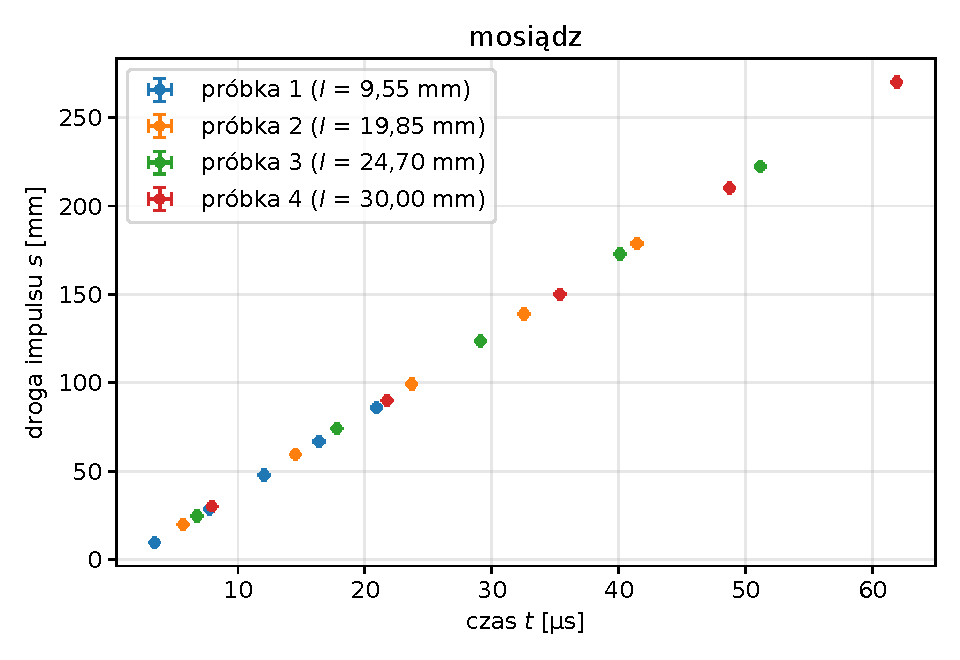
\includegraphics[width=0.75\textwidth]{brass_raw.pdf}
    \caption{Droga impulsu $s$ w~funkcji czasu $t$ dla próbek z~mosiądzu (1--4). Słupki błędów
             odpowiadają niepewnościom $u_t = 0{,}1$~µs i~$u(s) = (2n-1)\,u_l \le 0{,}45$~mm
             i~są mniejsze od znaczników.}
    \label{fig:brass_raw}
\end{figure}

\begin{figure}[H]
    \centering
    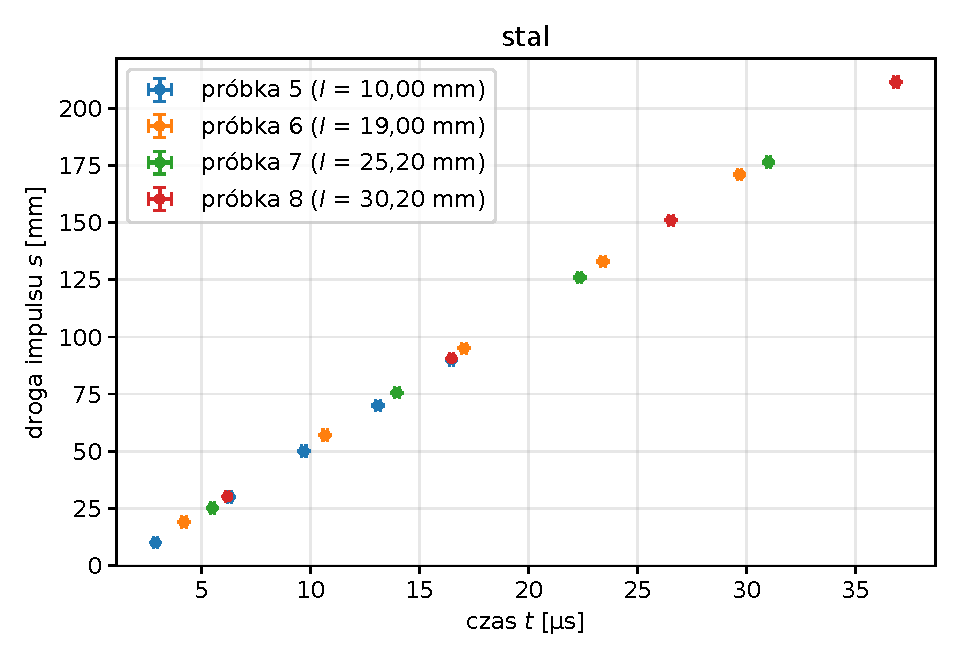
\includegraphics[width=0.75\textwidth]{steel_raw.pdf}
    \caption{Droga impulsu $s$ w~funkcji czasu $t$ dla próbek ze stali (5--8). Słupki błędów
             jak na Rysunku~\ref{fig:brass_raw}.}
    \label{fig:steel_raw}
\end{figure}

\begin{figure}[H]
    \centering
    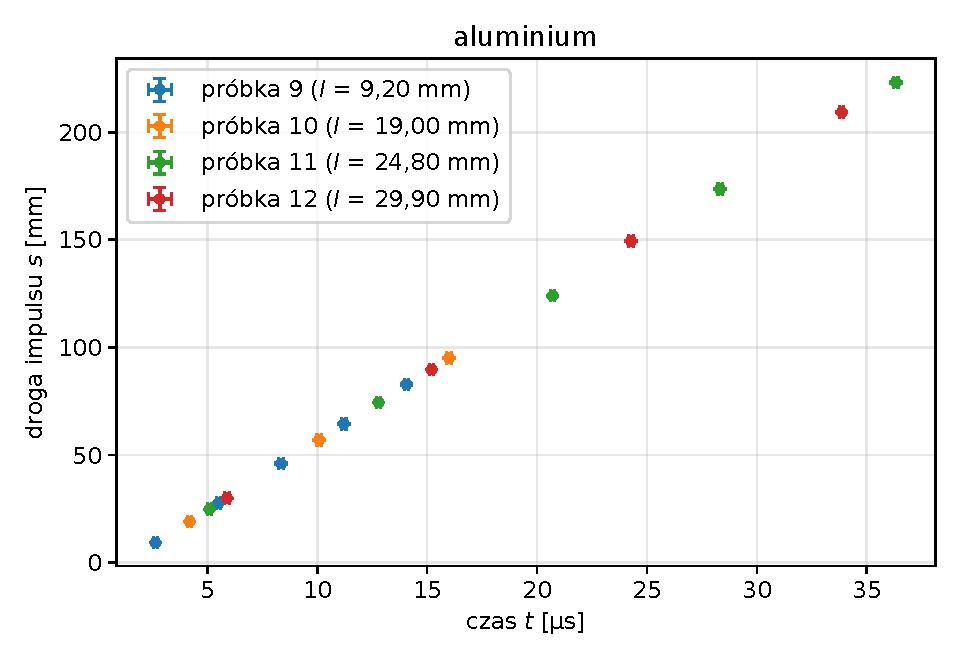
\includegraphics[width=0.75\textwidth]{aluminium_raw.pdf}
    \caption{Droga impulsu $s$ w~funkcji czasu $t$ dla próbek z~aluminium (9--12). Słupki
             błędów jak na Rysunku~\ref{fig:brass_raw}.}
    \label{fig:aluminium_raw}
\end{figure}



% -------------------------------------------
\section{Opracowanie wyników}
% -------------------------------------------

Wszystkie testy zgodności liczono z~niezaokrąglonych wartości; obliczenie z~liczb podanych
w~tekście może dać nieco inny wynik.

\subsection{Prędkość dźwięku}
\label{sec:predkosc}

\paragraph{Dopasowanie dla każdej próbki.}
Dla każdej próbki $i$ do punktów $\bigl((2n-1),\,t_n\bigr)$ dopasowano prostą~\eqref{eq:prosta}
$t_n = \tau_i(2n-1) + \delta_i$, gdzie $\tau_i$ --- czas przejścia impulsu przez grubość
próbki, $\delta_i$ --- opóźnienie układu dla tej próbki. Wartości $(2n-1)$ są dokładne,
a niepewność ma tylko $t_n$, dlatego zastosowano ważoną regresję liniową z~wagami
$w_n = 1/u_t^2$ (\texttt{scipy.optimize.curve\_fit} z~\texttt{sigma}~$=u_t$,
\texttt{absolute\_sigma=True}); niepewności parametrów to $u_\tau = \sqrt{C_{11}}$,
$u_\delta = \sqrt{C_{22}}$, gdzie $C$ --- macierz kowariancji. Dla próbek, w~których
$\chi^2/\nu_\text{sw} > 1$ (próbki 4 i~12), niepewności parametrów pomnożono przez
$\sqrt{\chi^2/\nu_\text{sw}}$ (2,38 i~1,57), żeby większy rozrzut ich punktów zmniejszał ich wagę
w~średniej. Prędkość w~próbce wynosi
$v_i = l_i/\tau_i$, a jej niepewność z~prawa propagacji niepewności
\begin{equation}
    \frac{u(v_i)}{v_i} = \sqrt{\left(\frac{u_\tau}{\tau_i}\right)^2 + \left(\frac{u_l}{l_i}\right)^2}.
    \label{eq:u_vi}
\end{equation}
Błąd pomiaru grubości $l_i$ przesuwa jednakowo drogi wszystkich impulsów danej próbki, dlatego
$u_l$ wchodzi do $u(v_i)$ raz, a nie osobno dla każdego punktu. Wyniki zestawiono
w~Tabeli~\ref{tab:probki_fit}, a dopasowane proste z~residuami przedstawiono na
Rysunkach~\ref{fig:brass_fit}--\ref{fig:aluminium_fit} (we współrzędnych $s(t)$, w~których
prosta próbki $i$ ma postać $s = v_i(t - \delta_i)$).

\begin{table}[H]
    \centering
    \caption{Prędkość $v_i$ i~opóźnienie $\delta_i$ z~dopasowania prostej~\eqref{eq:prosta}
             do punktów pojedynczej próbki oraz $\chi^2$ na liczbę stopni swobody $\nu_\text{sw}$.
             Niepewności dla próbek 4 i~12 przeskalowano przez $\sqrt{\chi^2/\nu_\text{sw}}$.}
    \label{tab:probki_fit}
    \begin{tabular}{cl S[table-format=4.0]@{\,$\pm$\,}S[table-format=2.0]
                      S[table-format=1.2]@{\,$\pm$\,}S[table-format=1.2] c}
        \toprule
        Nr & Materiał & \multicolumn{2}{c}{$v_i$ [m/s]} & \multicolumn{2}{c}{$\delta_i$ [µs]}
           & $\chi^2/\nu_\text{sw}$ \\
        \midrule
        1  & mosiądz   & 4380 & 39 & 1.22 & 0.09 & 2,03/3 \\
        2  & mosiądz   & 4433 & 19 & 1.19 & 0.09 & 2,53/3 \\
        3  & mosiądz   & 4446 & 16 & 1.22 & 0.09 & 2,18/3 \\
        4  & mosiądz   & 4445 & 26 & 1.41 & 0.22 & 16,95/3 \\
        \midrule
        5  & stal      & 5889 & 62 & 1.21 & 0.09 & 0,02/3 \\
        6  & stal      & 5964 & 33 & 1.08 & 0.09 & 1,32/3 \\
        7  & stal      & 5933 & 33 & 1.22 & 0.10 & 1,52/2 \\
        8  & stal      & 5919 & 28 & 1.11 & 0.10 & 1,19/2 \\
        \midrule
        9  & aluminium & 6454 & 80 & 1.23 & 0.09 & 0,02/3 \\
        10 & aluminium & 6441 & 79 & 1.25 & 0.12 & 0,01/1 \\
        11 & aluminium & 6361 & 29 & 1.16 & 0.09 & 2,90/3 \\
        12 & aluminium & 6434 & 50 & 1.22 & 0.16 & 4,92/2 \\
        \bottomrule
    \end{tabular}
\end{table}

\begin{figure}[H]
    \centering
    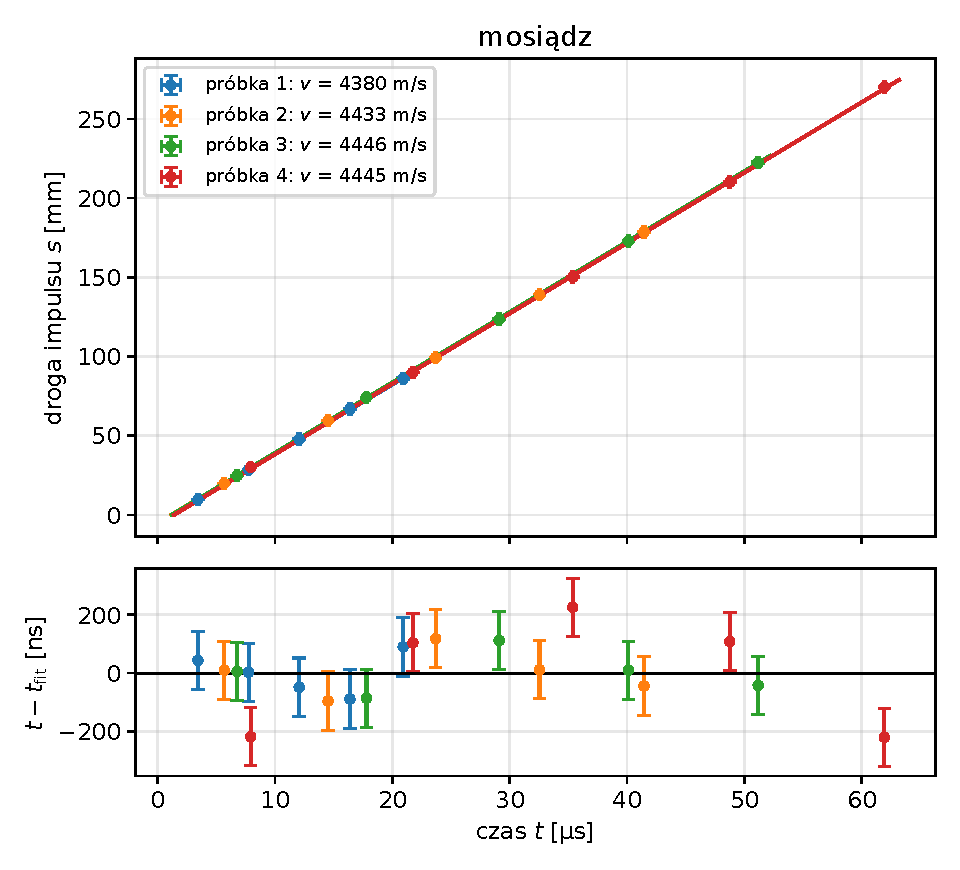
\includegraphics[width=0.72\textwidth]{brass.pdf}
    \caption{Droga impulsu $s$ w~funkcji czasu $t$ dla próbek mosiądzu z~prostymi dopasowanymi
             osobno do każdej próbki (u~góry) i~residua czasu $t - t_\text{fit}$ (u~dołu).
             Słupki błędów residuów odpowiadają $u_t = 0{,}1$~µs.}
    \label{fig:brass_fit}
\end{figure}

\begin{figure}[H]
    \centering
    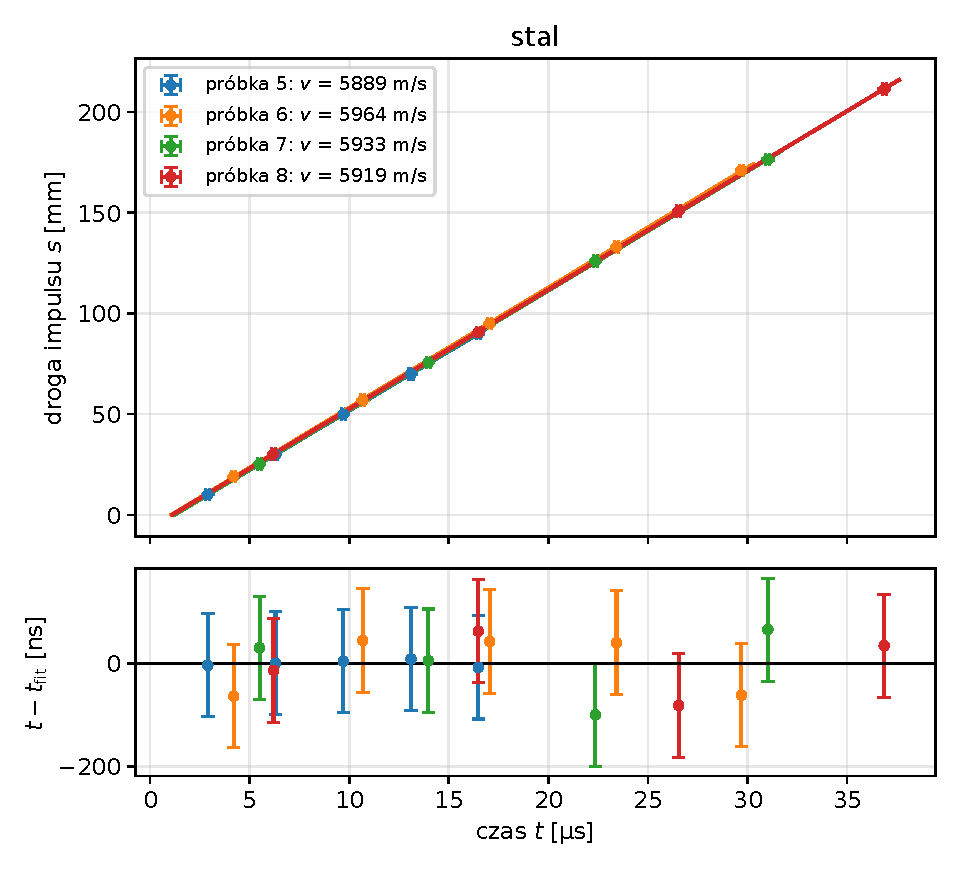
\includegraphics[width=0.72\textwidth]{steel.pdf}
    \caption{Droga impulsu $s$ w~funkcji czasu $t$ dla próbek stali z~prostymi dopasowanymi
             do każdej próbki i~residua. Oznaczenia jak na Rysunku~\ref{fig:brass_fit}.}
    \label{fig:steel_fit}
\end{figure}

\begin{figure}[H]
    \centering
    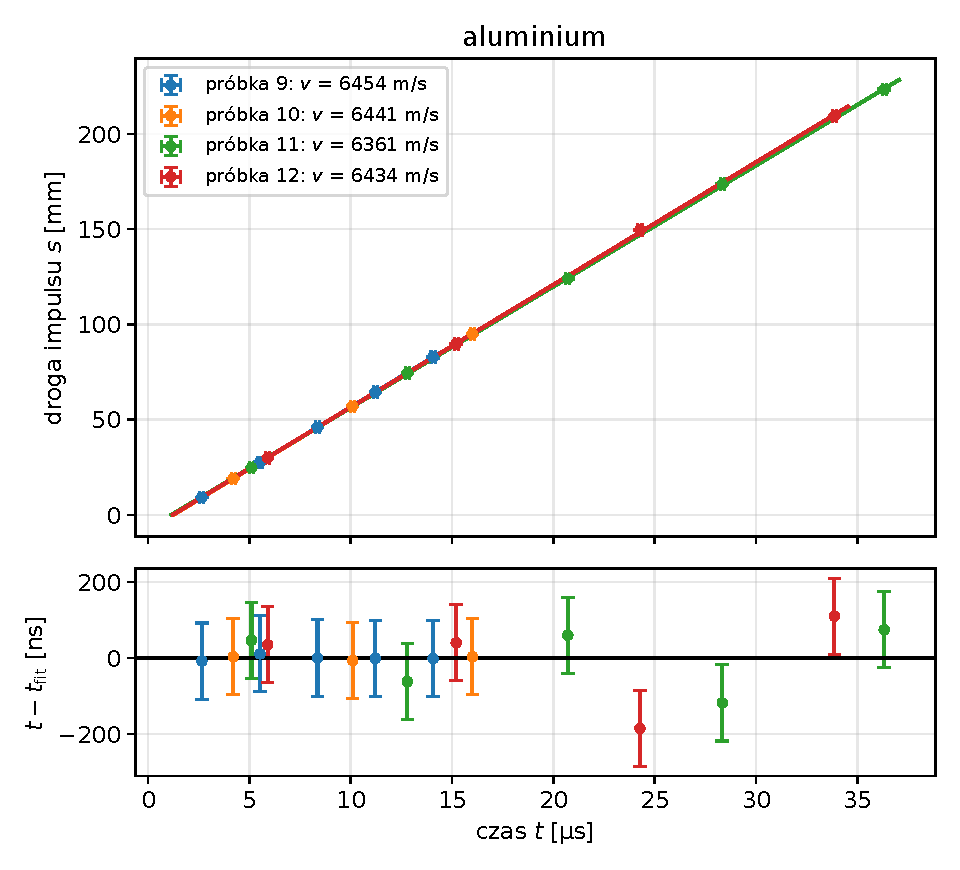
\includegraphics[width=0.72\textwidth]{aluminium.pdf}
    \caption{Droga impulsu $s$ w~funkcji czasu $t$ dla próbek aluminium z~prostymi dopasowanymi
             do każdej próbki i~residua. Oznaczenia jak na Rysunku~\ref{fig:brass_fit}.}
    \label{fig:aluminium_fit}
\end{figure}

\paragraph{Niepewność odczytu czasu.}
Łącznie dla 12 próbek $\sum\chi^2 = 35{,}6$ przy 31 stopniach swobody, a odchylenie
standardowe residuów czasu wewnątrz próbek wynosi 107~ns, więc przyjęta niepewność
$u_t = 0{,}1$~µs opisuje rozrzut odczytów. Jakość odczytów jest jednak niejednorodna: dla
próbek 5, 9 i~10 $\chi^2 \approx 0$ (czasy dokładne do kilku nanosekund), a dla próbki 4
$\chi^2 = 17{,}0$ przy 3 stopniach swobody. W~próbce 4 kolejne odstępy $t_{n+1} - t_n$ maleją
monotonicznie od 13,82 do 13,17~µs, a residua sięgają $\pm 0{,}2$~µs.

\paragraph{Opóźnienie układu.}
Opóźnienia $\delta_i$ wynoszą 1,08--1,41~µs. Różnice między próbkami są porównywalne
z~niepewnościami (0,09--0,22~µs), ale model z~osobnym $\delta_i$ nie zakłada, że są zerowe.

\paragraph{Przypisanie drogi.}
To, że $t_1$ odpowiada impulsowi bezpośredniemu (droga $l$), a nie pierwszemu echu (droga $2l$),
sprawdzono, dopasowując wspólną prostą $s(t)$ do wszystkich punktów danego materiału dla obu
przypisań. Przy $s_n = (2n-1)\,l$ otrzymano $\chi^2/\nu_\text{sw} = 29/18$, $20/16$ i~$14/15$
(mosiądz, stal, aluminium), a przy $s_n = 2nl$ --- $2970/18$, $1843/16$ i~$1528/15$: punkty
różnych próbek nie układają się wtedy na żadnej wspólnej prostej.

\paragraph{Prędkość materiału.}
Prędkość dla materiału obliczono jako średnią ważoną po próbkach,
\begin{equation}
    \bar v = \frac{\sum_i v_i/u^2(v_i)}{\sum_i 1/u^2(v_i)}, \qquad
    u(\bar v) = \left(\sum_i \frac{1}{u^2(v_i)}\right)^{-1/2},
    \label{eq:sr_waz}
\end{equation}
otrzymując
\begin{equation*}
    v_\text{mosiądz} = (4437 \pm 11)~\text{m/s}, \qquad
    v_\text{stal} = (5932 \pm 17)~\text{m/s}, \qquad
    v_\text{Al} = (6390 \pm 23)~\text{m/s},
\end{equation*}
z~$\chi^2 = 2{,}6$; $1{,}6$ i~$2{,}9$ przy 3 stopniach swobody, czyli prędkości z~poszczególnych
próbek są ze sobą zgodne (Rysunek~\ref{fig:velocities}). Nie uwzględniono wspólnego dla
wszystkich próbek błędu skali suwmiarki, który przesuwałby wszystkie prędkości proporcjonalnie.

\begin{figure}[H]
    \centering
    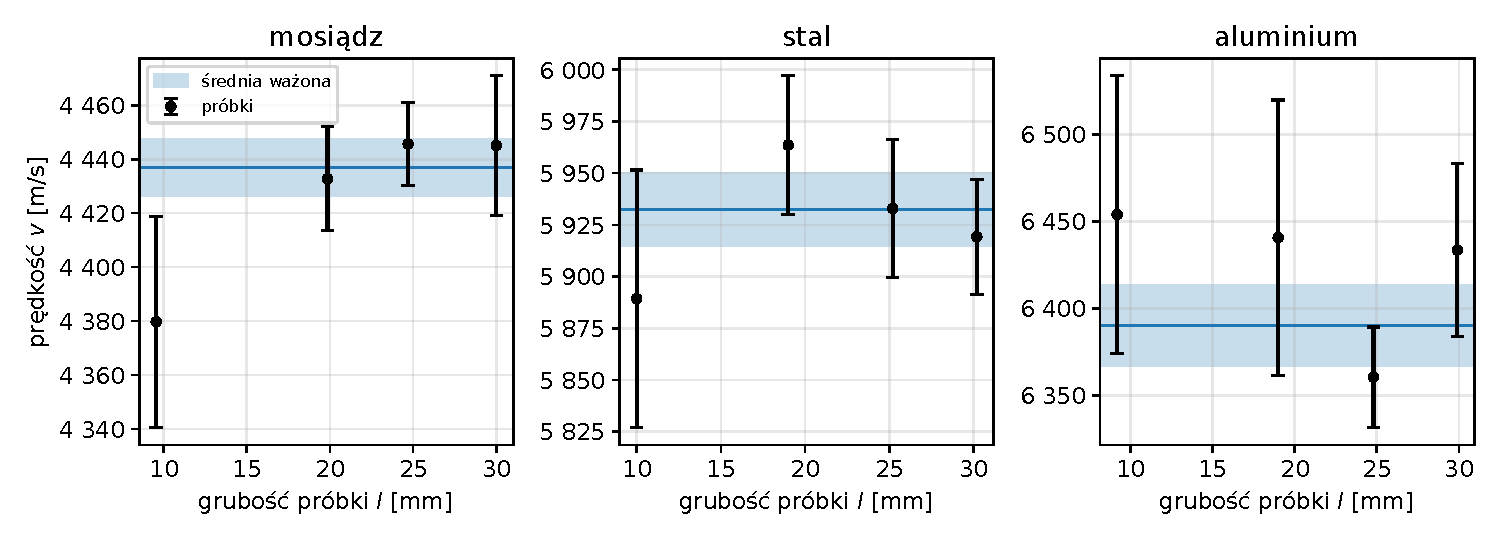
\includegraphics[width=0.95\textwidth]{velocities.pdf}
    \caption{Prędkości $v_i$ wyznaczone dla poszczególnych próbek w~funkcji ich grubości.
             Pas oznacza średnią ważoną $\bar v \pm u(\bar v)$, słupki błędów --- $u(v_i)$
             (wzór~\eqref{eq:u_vi}).}
    \label{fig:velocities}
\end{figure}

Najcieńsze próbki (1, 5, 9) mają też najmniejszą średnicę: $18{,}90$--$20{,}00$~mm wobec
$24{,}15$--$25{,}15$~mm pozostałych. Ich prędkości różnią się od średniej z~pozostałych trzech
próbek o~$-1{,}4$; $-0{,}8$ i~$+1{,}1\,\%$, czyli o~najwyżej $1{,}5\,\sigma$ --- w~zakresie
średnic 19--25~mm prędkość nie zależy od średnicy próbki.

\paragraph{Porównanie z~teorią.}
Prędkości przewidywane przez wzory~\eqref{eq:u_pret} (pręt) i~\eqref{eq:u_osr} (ośrodek
o~dużych rozmiarach poprzecznych) obliczono z~$E$ i~$\rho$ z~Tabeli~\ref{tab:tablica},
z~niepewnością
\begin{equation}
    \frac{u(v_\text{teor})}{v_\text{teor}} = \frac{1}{2}\sqrt{\left(\frac{u_E}{E}\right)^2
    + \left(\frac{u_\rho}{\rho}\right)^2 + \left(\frac{\mathrm{d}\ln f}{\mathrm{d}\nu}\,u_\nu\right)^2},
    \qquad
    \frac{\mathrm{d}\ln f}{\mathrm{d}\nu} = \frac{2}{1 - 2\nu} - \frac{1}{1 + \nu} - \frac{1}{1 - \nu},
    \label{eq:u_teor}
\end{equation}
przy czym ostatni składnik pod pierwiastkiem występuje tylko dla wzoru~\eqref{eq:u_osr}.
Wyniki zestawiono w~Tabeli~\ref{tab:teoria}, razem z~wartością ze skryptu i~wartościami
literaturowymi dla fali w~ośrodku nieograniczonym i~w~pręcie~\cite{sound}, którym przypisano
$u(v) = 5$~m/s (połowa ostatniej cyfry).

\begin{table}[H]
    \centering
    \footnotesize
    \caption{Zmierzona prędkość fali podłużnej $\bar v$ i~wartości teoretyczne: ze wzoru dla
             pręta~\eqref{eq:u_pret} i~dla ośrodka~\eqref{eq:u_osr} (z~$E$, $\rho$, $\nu$
             z~Tabeli~\ref{tab:tablica}), ze skryptu~\cite{skrypt} i~z~literatury~\cite{sound}.
             W~nawiasach test zgodności $|\bar v - v_\text{teor}|/\sqrt{u^2(\bar v) + u^2(v_\text{teor})}$.
             Wszystkie prędkości w~m/s.}
    \label{tab:teoria}
    \begin{tabular}{lccccc}
        \toprule
        Materiał & $\bar v$ & pręt~\eqref{eq:u_pret} & ośrodek~\eqref{eq:u_osr}
                 & skrypt & literatura: ośrodek / pręt \\
        \midrule
        mosiądz   & $4437 \pm 11$ & $3566 \pm 14$ (49,7)  & $4424 \pm 177$ (0,1) & $3830 \pm 5$ (52,0)  & $4700 \pm 5$ (22,6) / $3480 \pm 5$ \\
        stal      & $5932 \pm 17$ & $5250 \pm 18$ (27,4)  & $6010 \pm 156$ (0,5) & $5950 \pm 50$ (0,3)  & $5940 \pm 5$ (0,4) / $5180 \pm 5$ \\
        aluminium & $6390 \pm 23$ & $5000 \pm 209$ (6,6)  & $6086 \pm 337$ (0,9) & $6320 \pm 5$ (3,0)   & $6420 \pm 5$ (1,3) / $5000 \pm 5$ \\
        \bottomrule
    \end{tabular}
\end{table}

Dla wszystkich trzech materiałów zmierzona prędkość jest zgodna ze wzorem~\eqref{eq:u_osr}
(test $\le 0{,}9$) i~niezgodna ze wzorem~\eqref{eq:u_pret} (test $6{,}6$--$49{,}7$).
Z~wartością ze skryptu zgodny jest wynik dla stali ($0{,}3$); dla aluminium test wynosi $3{,}0$,
a dla mosiądzu $52{,}0$.

Prędkości podane w~skrypcie porównano też z~prędkościami obliczonymi z~$E$ i~$\rho$ z~tej samej
tabeli. Dla stali i~aluminium są one zgodne z~wzorem dla ośrodka~\eqref{eq:u_osr} (test $0{,}4$
i~$0{,}7$) i~o~13 oraz 26\,\% większe od prędkości w~pręcie. Wartość dla mosiądzu, 3830~m/s, nie odpowiada
żadnemu z~wzorów: jest o~7\,\% większa od prędkości w~pręcie (3566~m/s) i~o~13\,\% mniejsza
od prędkości w~ośrodku ($(4424 \pm 177)$~m/s, test $3{,}3$).

\subsection{Gęstość}

Gęstość każdej próbki obliczono ze wzoru~\eqref{eq:rho}, z~niepewnością
\begin{equation}
    \frac{u(\rho)}{\rho} = \sqrt{\left(\frac{u_m}{m}\right)^2 + \left(\frac{2u_d}{d}\right)^2
    + \left(\frac{u_l}{l}\right)^2}.
    \label{eq:u_rho}
\end{equation}
Wyniki zestawiono w~Tabeli~\ref{tab:rho}.

\begin{table}[H]
    \centering
    \caption{Gęstości próbek obliczone ze wzoru~\eqref{eq:rho}.}
    \label{tab:rho}
    \begin{tabular}{cl S[table-format=4.0]@{\,$\pm$\,}S[table-format=2.0]}
        \toprule
        Nr & Materiał & \multicolumn{2}{c}{$\rho$ [kg/m$^3$]} \\
        \midrule
        1  & mosiądz   & 8532 & 64 \\
        2  & mosiądz   & 8333 & 40 \\
        3  & mosiądz   & 8411 & 38 \\
        4  & mosiądz   & 8375 & 36 \\
        \midrule
        5  & stal      & 7955 & 57 \\
        6  & stal      & 7789 & 37 \\
        7  & stal      & 7800 & 36 \\
        8  & stal      & 7817 & 34 \\
        \midrule
        9  & aluminium & 2827 & 21 \\
        10 & aluminium & 2798 & 13 \\
        11 & aluminium & 2798 & 13 \\
        12 & aluminium & 2787 & 12 \\
        \bottomrule
    \end{tabular}
\end{table}

W~każdym materiale najwyższą gęstość daje najcieńsza próbka (1, 5 i~9): o~1,9; 2,0 i~1,2\,\%
więcej niż średnia pozostałych trzech. Z~tego powodu średnia ważona miałaby
$\chi^2 = 7{,}5$; $6{,}7$ i~$2{,}6$ przy 3 stopniach swobody, a jej niepewność
(21, 19 i~7~kg/m$^3$) nie obejmowałaby rozrzutu między próbkami. Dlatego gęstość materiału
obliczono jako średnią arytmetyczną $\bar\rho$ czterech próbek z~niepewnością równą
odchyleniu standardowemu średniej,
\begin{equation}
    u(\bar\rho) = \sqrt{\frac{1}{n(n-1)}\sum_{i=1}^{n}\left(\rho_i - \bar\rho\right)^2}, \qquad n = 4,
    \label{eq:u_sr}
\end{equation}
otrzymując
\begin{equation*}
    \rho_\text{mosiądz} = (8413 \pm 43)~\text{kg/m}^3, \qquad
    \rho_\text{stal} = (7840 \pm 39)~\text{kg/m}^3, \qquad
    \rho_\text{Al} = (2802 \pm 9)~\text{kg/m}^3.
\end{equation*}
Wartości te są większe od wartości ze skryptu~\cite{skrypt} o~3,9; 0,5 i~3,8\,\%; test
zgodności wynosi $4{,}8$ dla mosiądzu, $0{,}6$ dla stali i~$2{,}0$ dla aluminium.

\subsection{Moduł podłużny i~moduł Younga}

Moduł podłużny obliczono ze wzoru~\eqref{eq:M}, a moduł Younga ze wzoru~\eqref{eq:E},
z~niepewnościami
\begin{equation}
    \frac{u(M)}{M} = \sqrt{\left(\frac{u(\bar\rho)}{\bar\rho}\right)^2 + \left(\frac{2\,u(\bar v)}{\bar v}\right)^2},
    \qquad
    \frac{u(E)}{E} = \sqrt{\left(\frac{u(M)}{M}\right)^2
    + \left(\frac{\mathrm{d}\ln f}{\mathrm{d}\nu}\,u_\nu\right)^2}.
    \label{eq:u_E}
\end{equation}
Wyniki zestawiono w~Tabeli~\ref{tab:E}.

\begin{table}[H]
    \centering
    \caption{Moduł podłużny $M = \bar\rho\bar v^2$, moduł Younga $E = M/f(\nu)$, wartość tablicowa
             $E_\text{tab}$~\cite{skrypt} i~test zgodności $|E - E_\text{tab}|/\sqrt{u^2(E) + u^2(E_\text{tab})}$.}
    \label{tab:E}
    \begin{tabular}{l S[table-format=2.2]@{\,$\pm$\,}S[table-format=1.2] c
                      S[table-format=2.2]@{\,$\pm$\,}S[table-format=1.2] c c}
        \toprule
        Materiał & \multicolumn{2}{c}{$M$ [$10^{10}$ Pa]} & $f(\nu)$
                 & \multicolumn{2}{c}{$E$ [$10^{10}$ Pa]} & $E_\text{tab}$ [$10^{10}$ Pa] & test \\
        \midrule
        mosiądz   & 16.56 & 0.12 & 1,54 & 10.76 & 0.86 & 10,3     & 0,5 \\
        stal      & 27.59 & 0.21 & 1,31 & 21.06 & 1.10 & 21,5     & 0,4 \\
        aluminium & 11.44 & 0.09 & 1,48 & 7.72  & 0.57 & 6,2--7,3 & 1,2 \\
        \bottomrule
    \end{tabular}
\end{table}

Moduł podłużny wyznaczono z~niepewnością 0,7--0,8\,\%. Moduł Younga jest zgodny z~wartościami
tablicowymi dla wszystkich materiałów, ale jego niepewność w~98--99\,\% pochodzi
od $u_\nu$: wartość $E$ jest w~praktyce wyznaczona przez przyjęty współczynnik Poissona.
Przy $u_\nu/\sqrt{3}$ zamiast $u_\nu$ niepewności $E$ zmalałyby do $0{,}50$; $0{,}65$
i~$0{,}33 \cdot 10^{10}$~Pa, a testy zgodności wyniosłyby $0{,}9$; $0{,}7$ i~$1{,}5$.

% -------------------------------------------
\section{Wnioski}
% -------------------------------------------

\subsection{Prędkość dźwięku}

Wyznaczone prędkości fali podłużnej wynoszą $(4437 \pm 11)$~m/s dla mosiądzu,
$(5932 \pm 17)$~m/s dla stali i~$(6390 \pm 23)$~m/s dla aluminium. Wszystkie trzy są zgodne
z~prędkością fali w~ośrodku o~dużych rozmiarach poprzecznych, wzór~\eqref{eq:u_osr}
(test $0{,}1$; $0{,}5$ i~$0{,}9$), a niezgodne ze wzorem dla cienkiego pręta (test
$6{,}6$--$49{,}7$). Brak zależności prędkości od średnicy próbki (19--25~mm) jest zgodny
z~modelem ośrodka nieograniczonego, ale go nie rozstrzyga, bo obie średnice są wielokrotnie
większe od długości fali; głównym argumentem pozostaje porównanie ze wzorami~\eqref{eq:u_pret}
i~\eqref{eq:u_osr}. Wynik dla stali jest
zgodny z~wartością ze skryptu ($0{,}3$) i~z~literaturą ($0{,}4$~\cite{sound}).

Wynik dla mosiądzu nie jest zgodny z~wartością ze skryptu, 3830~m/s (test $52{,}0$). Przyczyną
jest sama wartość tablicowa: tabela skryptu jest wewnętrznie niespójna. Dla stali i~aluminium
podane prędkości odpowiadają fali w~ośrodku, obliczonej z~$E$ i~$\rho$ z~tej samej tabeli,
natomiast 3830~m/s dla mosiądzu nie odpowiada ani fali w~ośrodku ($4424 \pm 177$~m/s),
ani w~pręcie (3566~m/s). Zmierzona prędkość jest zgodna z~prędkością w~ośrodku obliczoną
z~$E$, $\rho$ i~$\nu$ mosiądzu (test $0{,}1$).

Wynik dla aluminium różni się od wartości ze skryptu, 6320~m/s, o~1,1\,\% (test $3{,}0$).
Prawdopodobną przyczyną jest inny materiał: zmierzona gęstość próbek, $(2802 \pm 9)$~kg/m$^3$, jest
o~3,8\,\% większa od gęstości czystego aluminium i~odpowiada stopom aluminium
($2770$--$2830$~kg/m$^3$~\cite{density}), a prędkość dźwięku zależy od stopu. Wynik jest
zgodny z~literaturową prędkością dla aluminium walcowanego, 6420~m/s ($1{,}3$~\cite{sound}),
i~z~prędkością obliczoną z~$E$ i~$\rho$ ze skryptu ($0{,}9$).

Rozrzut odczytów czasu (107~ns) potwierdza przyjętą niepewność $u_t = 0{,}1$~µs, ale jakość
odczytu zależała od próbki. W~próbce 4 odstępy między kolejnymi impulsami maleją monotonicznie
o~0,65~µs. Za moment dotarcia impulsu przyjmowano jego najwyższe maksimum, a kolejne echa są
coraz słabsze i~bardziej rozmyte, więc najwyższe maksimum przesuwa się w~obrębie impulsu
lub przeskakuje o~okres fali nośnej (rzędu 0,2--0,5~µs przy częstotliwościach
megahercowych). Odczyt tego samego przejścia przez zero we wszystkich echach usunąłby ten efekt.

\subsection{Gęstość}

Wyznaczone gęstości wynoszą $(8413 \pm 43)$~kg/m$^3$ dla mosiądzu, $(7840 \pm 39)$~kg/m$^3$
dla stali i~$(2802 \pm 9)$~kg/m$^3$ dla aluminium. Gęstości stali i~aluminium są zgodne
z~wartościami ze skryptu (test $0{,}6$ i~$2{,}0$).

Gęstość mosiądzu nie jest zgodna z~wartością ze skryptu, $8100$~kg/m$^3$ (test $4{,}8$).
Przyczyną jest wartość tablicowa: gęstość mosiądzu zależy od zawartości miedzi i~cynku
i~dla mosiądzów walcowanych i~lanych wynosi $8400$--$8730$~kg/m$^3$~\cite{density}. Wartość
ze skryptu leży poniżej tego przedziału, a zmierzona --- w~nim.

Najcieńsze próbki (1, 5, 9) dają we wszystkich materiałach gęstość wyższą o~1,2--2,0\,\% od
pozostałych. Ta sama nadwyżka wynikałaby z~zaniżenia ich średnicy o~0,1--0,2~mm albo grubości
o~0,1--0,2~mm, czyli 2--4 razy więcej niż $u_l = u_d = 0{,}05$~mm. Zaniżona grubość obniżyłaby
też prędkość, a prędkości najcieńszych próbek odchylają się od średniej w~obie strony
($-1{,}4$; $-0{,}8$; $+1{,}1\,\%$), co wskazuje raczej na średnicę, od której prędkość nie zależy.
Nawet gdyby grubość tych próbek była zaniżona o~1,5\,\%, średnie prędkości zmieniłyby się
o~5--8~m/s, mniej niż ich niepewności, bo najcieńsze próbki mają wagę 7--8\,\% w~średniej
ważonej.

\subsection{Moduł podłużny i~moduł Younga}

Bezpośrednio zmierzonym modułem sprężystości jest moduł podłużny: $(16{,}56 \pm 0{,}12)$,
$(27{,}59 \pm 0{,}21)$ i~$(11{,}44 \pm 0{,}09) \cdot 10^{10}$~Pa dla mosiądzu, stali i~aluminium.
Moduły Younga obliczone z~niego, $(10{,}76 \pm 0{,}86)$, $(21{,}06 \pm 1{,}10)$
i~$(7{,}72 \pm 0{,}57) \cdot 10^{10}$~Pa, są zgodne z~wartościami tablicowymi (test $0{,}5$;
$0{,}4$ i~$1{,}2$). Ta zgodność jest jednak w~dużej mierze zapewniona przez założenia: niepewność
$E$ w~98--99\,\% pochodzi z~niepewności współczynnika Poissona, przyjętego z~literatury dla
nieznanego gatunku materiału. Uniezależnienie $E$ od tablic wymagałoby pomiaru prędkości fali
poprzecznej, z~której stosunku do $v_\parallel$ wynika $\nu$ (wzór~\eqref{eq:nu}).


\begin{thebibliography}{9}
\bibitem{skrypt}
    \textit{Skrypt do ćwiczeń laboratoryjnych z~fizyki, I Pracownia Fizyczna}, ćwiczenie F9:
    Pomiar prędkości dźwięku w~metalach metodą echa ultradźwiękowego, Wydział Fizyki,
    Astronomii i~Informatyki Stosowanej, Uniwersytet Jagielloński, s.~198--203.
\bibitem{poisson}
    Engineering ToolBox, \textit{Poisson's Ratio},
    \url{https://www.engineeringtoolbox.com/poissons-ratio-d_1224.html}
    [dostęp: 10 listopada 2026]
\bibitem{sound}
    Engineering ToolBox, \textit{Solids and Metals --- Speed of Sound},
    \url{https://www.engineeringtoolbox.com/sound-speed-solids-d_713.html}
    [dostęp: 10 listopada 2026]
\bibitem{density}
    Engineering ToolBox, \textit{Metals and Alloys --- Densities},
    \url{https://www.engineeringtoolbox.com/metal-alloys-densities-d_50.html}
    [dostęp: 10 listopada 2026]
\end{thebibliography}

\end{document}
% =============================================
